\section{Experimental Evaluation}
\label{sec:experimentalevaluation}
We measure teh forecasting effectiveness on its abilities to predict the proton flux and if an SEP event occurs 30 (t+6) minutes and (t+12) minutes ahead.

\subsection{Evaluation of SEP Time-Intensity Profile Prediction}
\subsubsection{Evaluation Criteria}
We compute  mean absolute error (MAE) across all models and their predictions. We sum all errors at each timestep between the true versus predicted proton flux and take the mean.

\begin{align}
    MAE = \frac{1}{n}\sum |x_{\text{pred}}-x_{\text{true}}|
\end{align}

We measure the lag time of between the predicted and true proton flux. We shift our predicted protons between the onset and peak of each event align with the true protons and measure MAE at each shift. Once we have the minimum value of MAE we measure the time lag.

\begin{figure}[!htbp]
    \centering
    \includegraphics[width=0.7\textwidth,height=0.25\textheight,keepaspectratio]{figs/4.1.2 Learning and Evaluation Procedure/drawing_bootstrap example.png}
    \caption{Placeholder: will be replaced with real data showing background chunks and event chunks.}
    \label{fig:bootstrap_chunking}
\end{figure}

A third prediction efficiency metric is used as a comparison as well. For a discrete time series as

\begin{align}
  PE = 1 - \frac{SSR}{SST}
\end{align}

with $\langle . \rangle$ denoting arithmetic mean, $x_{\text{obs}}$ the observation, $x_{\text{mod}}$ the modeled signal, and $\sigma_{\text{obs}}^2$ as the variance in the observed signal. PE indicated perfect model performance and PE = 0 indicated performance comparable to predicting the arithmetic mean of the observed signal. PE can reach unlimited negative values. \cite{Rastatter2011PE}

An F1 score evaluates the performance of our forecasting model. The score is calculated by arithmetic operations of the number of true positive, false positives, and false negatives the solve into the recall \eqref{recall} and precision \eqref{precision}. the recall and precision values are then used to calculate our final F1 score \eqref{F1}:
\begin{equation}
    \label{recall}
    \text{recall} = \frac{TP}{TP + FN} 
\end{equation}
\begin{equation}
    \label{precision}
    \text{precision} = \frac{TP}{TP+FP}
\end{equation}
\begin{equation}
    \label{F1}
    \text{F1} = \frac{2 \times \text{precision} \times \text{recall}}{\text{precision} + \text{recall}}
\end{equation}.
\subsubsection{Learning and Evaluation Procedures}

In measure variability of our statistics we run ten blocked bootstraps experiments. A block bootstrap partitions the original data and resample the blocks in a shuffled order for a new time series dataset. This is different than a standard bootstrap since we want to preserve the loss of the electron - proton rising patterns necessary to make predictions. 

We first block from $t-36$ before the onset of each event to the end and slice them out. This leaves us with the background data left in the time series.  For this we choose a block size of $n^{1/3}$ where $n$ is the length of our time series data. \cite{bertail2024optimal}. Repeating this process nine times plus our original dataset, $d_0$, we are left with ten total datasets. 

\begin{figure}[!htbp]
    \centering
    \includegraphics[width=0.7\textwidth,height=0.25\textheight,keepaspectratio]{figs/4.1.2 Learning and Evaluation Procedure/drawing_bootstrap example.png}
    \caption{Placeholder: will be replaced with real data showing background chunks and event chunks.}
    \label{fig:bootstrap_chunking}
\end{figure}

Each dataset is split into training and testing portions with an 80/20 ratio. $d_0$ contains $21$ SEP events in the training split and $18$ in the test split. Bootstrapping randomly switches these events from train or test portions allowing forecasting models learn from all $39$ SEP events rather than $21$. Each machine learning model trains 10 models on each dataset totaling 100 models for one forecasting time lead $(t+6, t+12)$.

For each model and dataset we produce a sample for each metric. we assume a student-t distribution for a  small sample size and unknown variance. we choose a mean estimate for all samples to get a bootstrap estimate $\hat{\theta}$:
$$
\begin{align*}
    \hat{\theta}^* = \frac{1}{n} \sum_i^n \theta_i^*
\end{align*}
$$

For each metric measured from a model trained on a dataset we compute the mean bootstrap estimate

$$
\bar{\theta} = \frac{1}{B}\sum_i^B \hat{\theta}_i^*
$$

Where $B$ is the number of bootstrap estimates.

We retrieve the bias for the small sample size and the standard error:
$$
\begin{align*}
    S_{\hat{\theta}}^2 &= \frac{1}{B-1} \sum_i^B (\hat{\theta}_i^* - \bar{\theta}^*) ^2\\\\
    S_{b}^2 &= \frac{1}{B} \sum_i^B (\hat{\theta}_i^* - \bar{\theta}^*) ^2
\end{align*}
$$

A bootstrap confidence is calculated with a significance value of $\alpha = .05$:
$$
\begin{align*}
    CI = \left(\bar{\theta} - t_{\alpha/2} \frac{s_\theta}{\sqrt{n}} , \bar{\theta} + t_{\alpha/2} \frac{s_\theta}{\sqrt{n}} \right)
\end{align*}
$$

 A Welch -T Test compares the mean performance of each champion model to baseline model.
 $$
 \begin{align*}
     \text{t-stat} = \frac{(\bar{x}_{base} - \bar{x}_\text{champ}) - (\bar{\mu}_{base} - \bar{\mu}_\text{champ})}{\sqrt{\frac{s_{\text{base}}}{n_\text{base}}+\frac{s_{\text{champ}}}{n_\text{champ}}}}
 \end{align*}
 $$

\subsubsection{Torres Machine Learning Model}
To properly compare our transformer model with RNN and NN models we train the transformer to minimizes loss by the mean square error (MSE) in log space between the target proton intensity and the predicted proton intensity. The output will also be in natural logarithm space \cite{torres2025machine}.

To match the RNN and NN, weights are updated using Adam optimizer and we converge if the loss function does not change by more the $10^{-4}$ over 20 iterations. We train five separate models at different seeds $(1-5)$ and average and standard deviation of MAE and lag \cite{torres2025machine}.



\subsubsection{Baseline Methods Used for Comparison}
\cite{torres2025machine} uses a persistent model as a baseline for their RNN and NN models. its a simple baseline method in which the predicted proton flux value is the current proton flux value, which is equivalent to now cast. \cite{posner2007forecasting} matrix will be compared to as well across the same metrics.

A linear regression model implemented from pythons SkLearn library will also be used as a baseline for our transformer

The baseline models are deterministic so we will only report a single run

\subsubsection{Results}

We compare the performance of our models to the different methods offered by Torres for t+6 and t+12 in Figure \ref{fig:mae_lag_comparison}. For both t+6 and t+12 we see similar behavior. All models of different architecture (Rope, Sinusoidal, Zero Init) slightly outperforms Torres's RNN and NN for MAE at both $t+6$ and $t+12$ Neural network models have more fluctuation in their predictions which can yield larger vertical gaps, particularity when the proton flux is relatively flat or slow rising \cite{torres2025machine}.

Lag, however, tends to measure larger. Torres explained their lag problem underperformed \cite{posner2007forecasting} forecasting matrix as the method over predicts proton intensity. Reducing the lag in the forecasting was hoped to be solved by a transformer. 


\begin{figure}[!htbp]
    \centering
    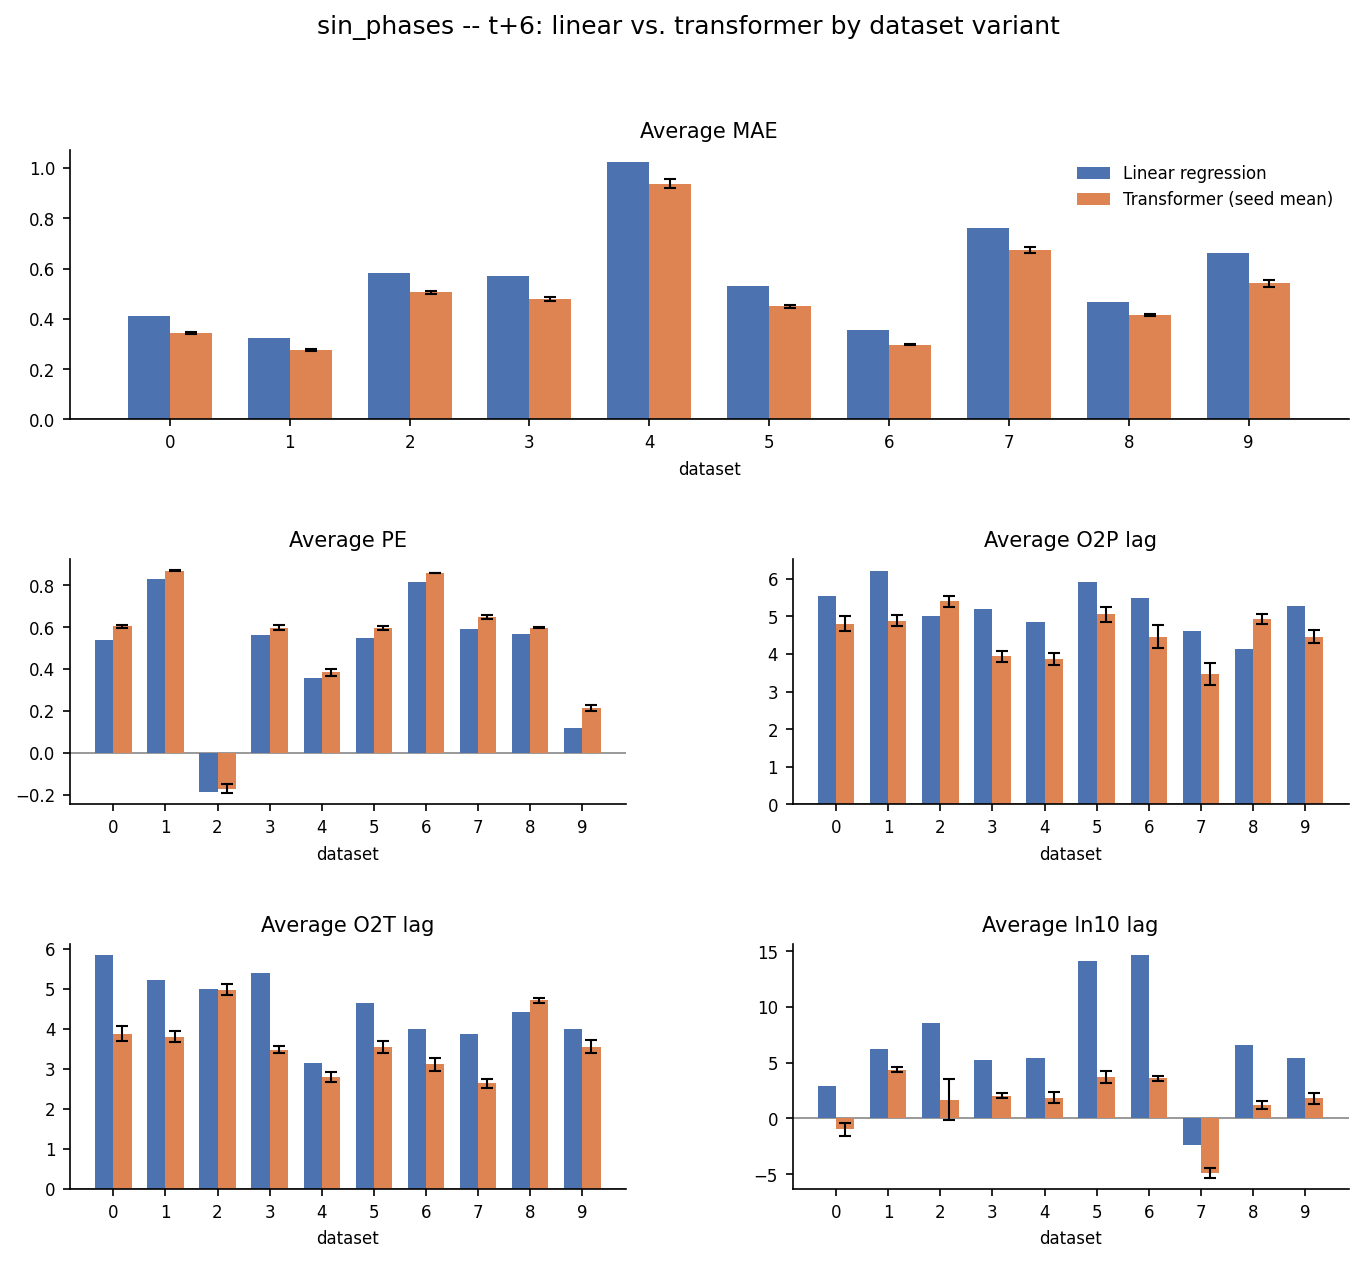
\includegraphics[width=0.7\textwidth]{plots/sin_phases_t6_linear_vs_transformer.png}
    \caption{This image is from real results from my cross validation split of 10 datasets but only for my sin encoded transformer. incomplete but wanted to show this here for now.}
    \label{fig:sinusoidal_t6_comparison}
\end{figure}

\begin{figure}[!htbp]
    \centering
    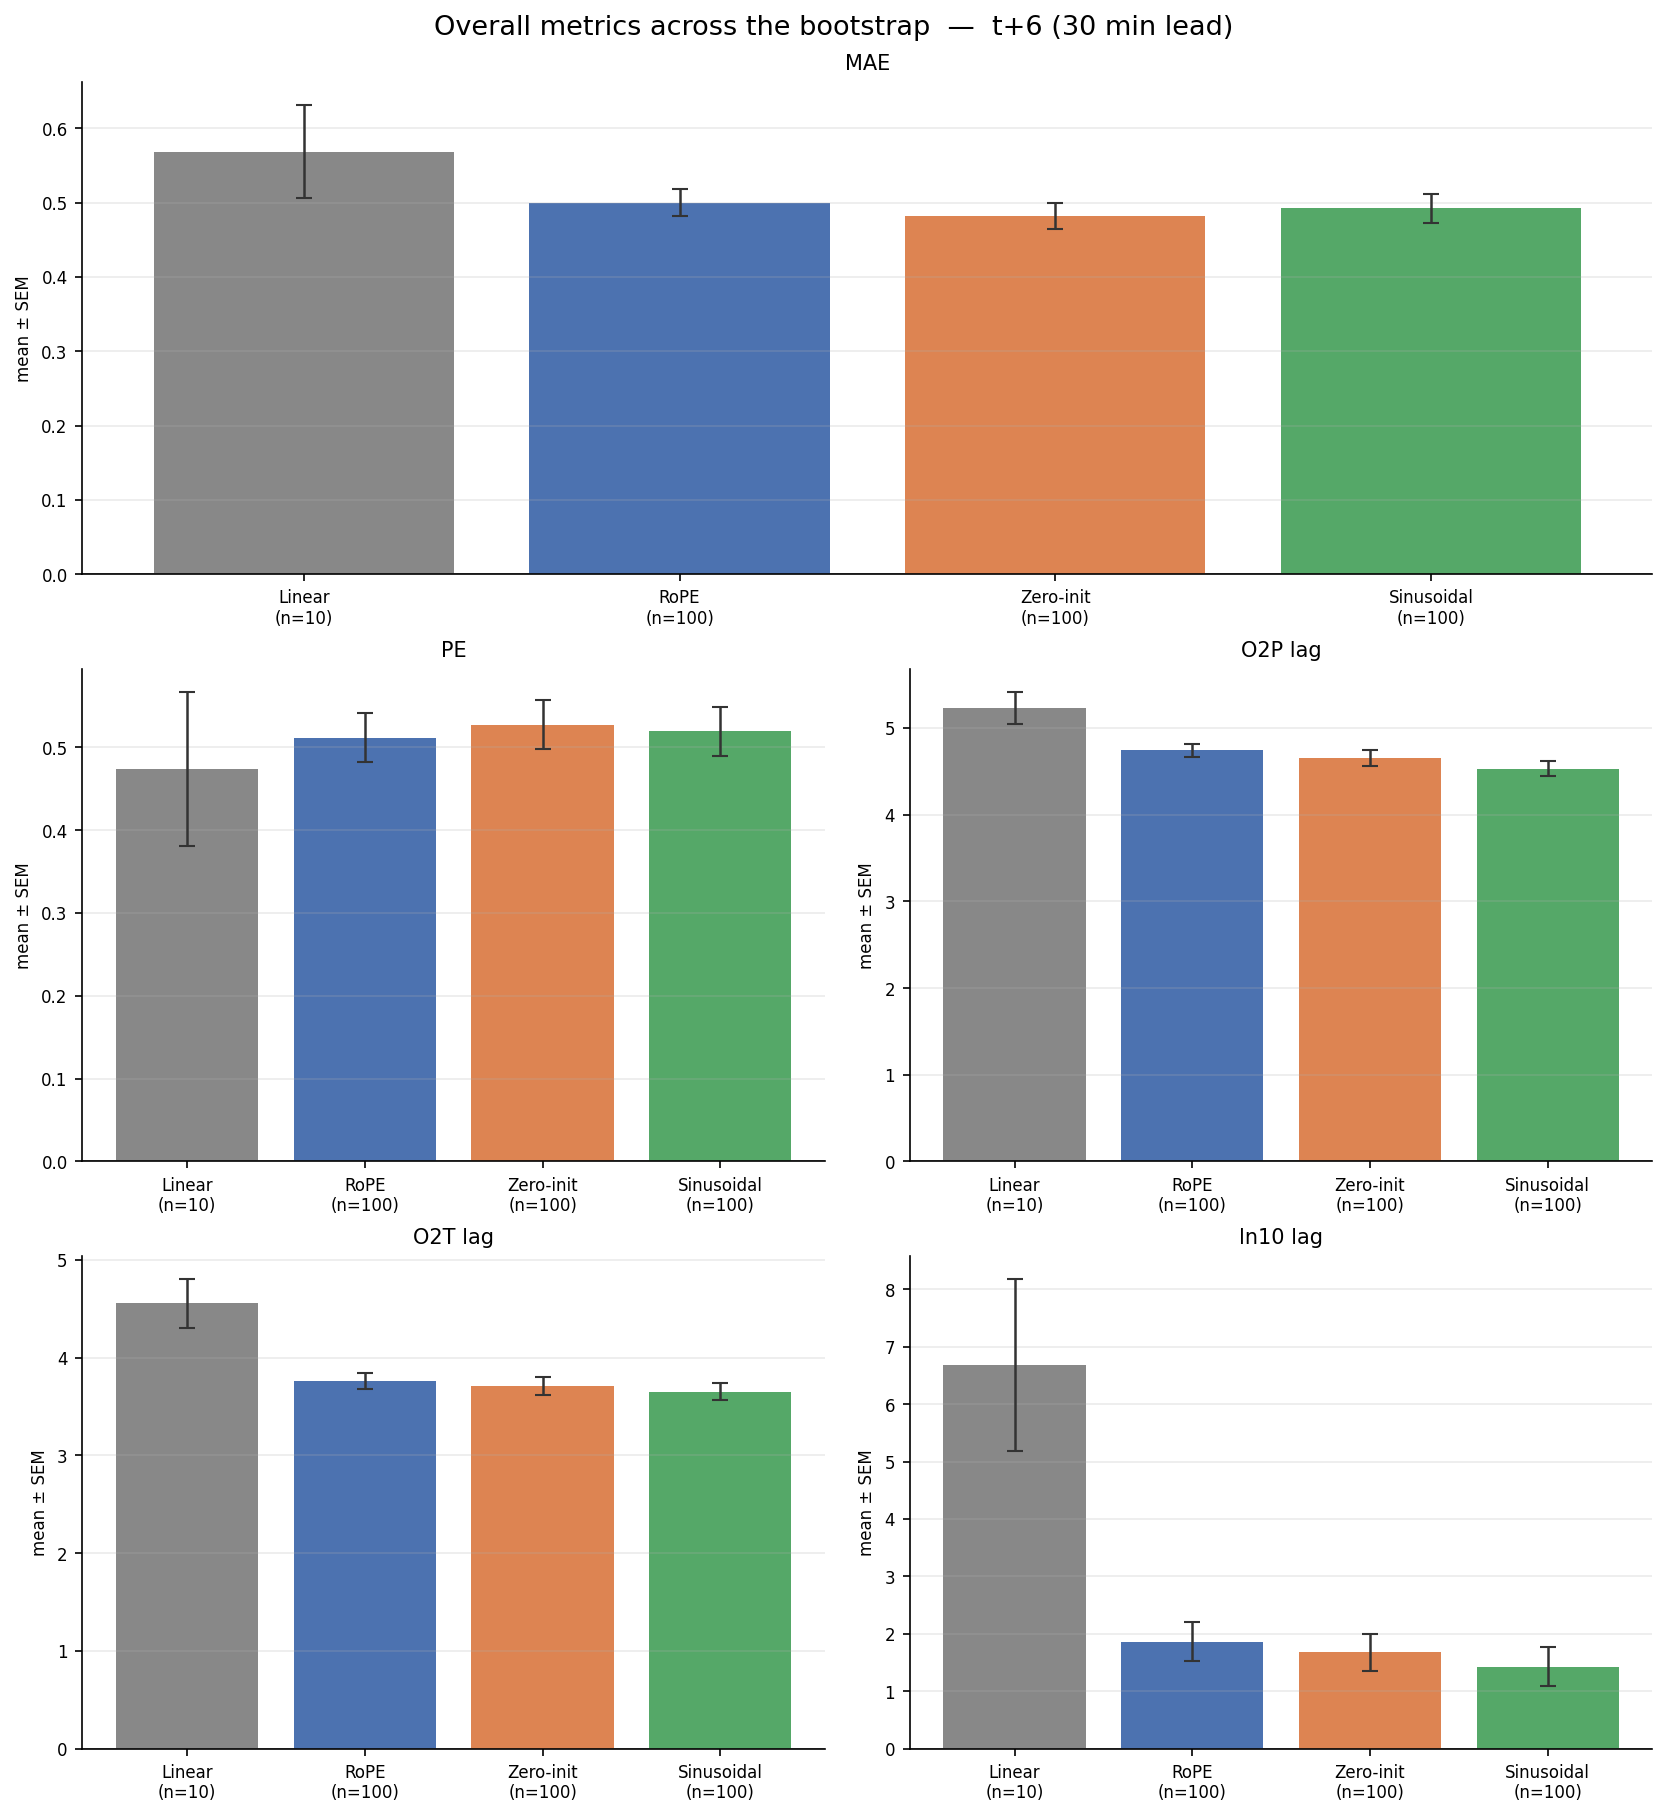
\includegraphics[width=0.7\textwidth]{plots/overall_comparison_t+6.png}
    \caption{Bootstrap of Rope,Sin and Zero init models compared with linear regression  MAE, Lags and Predictive efficiencies with forecasting time of 30 minutes w/ phases TODO add torres nn and rnn}
    \label{fig:sinusoidal_t6_comparison}
\end{figure}
\begin{figure}[!htbp]
    \centering
    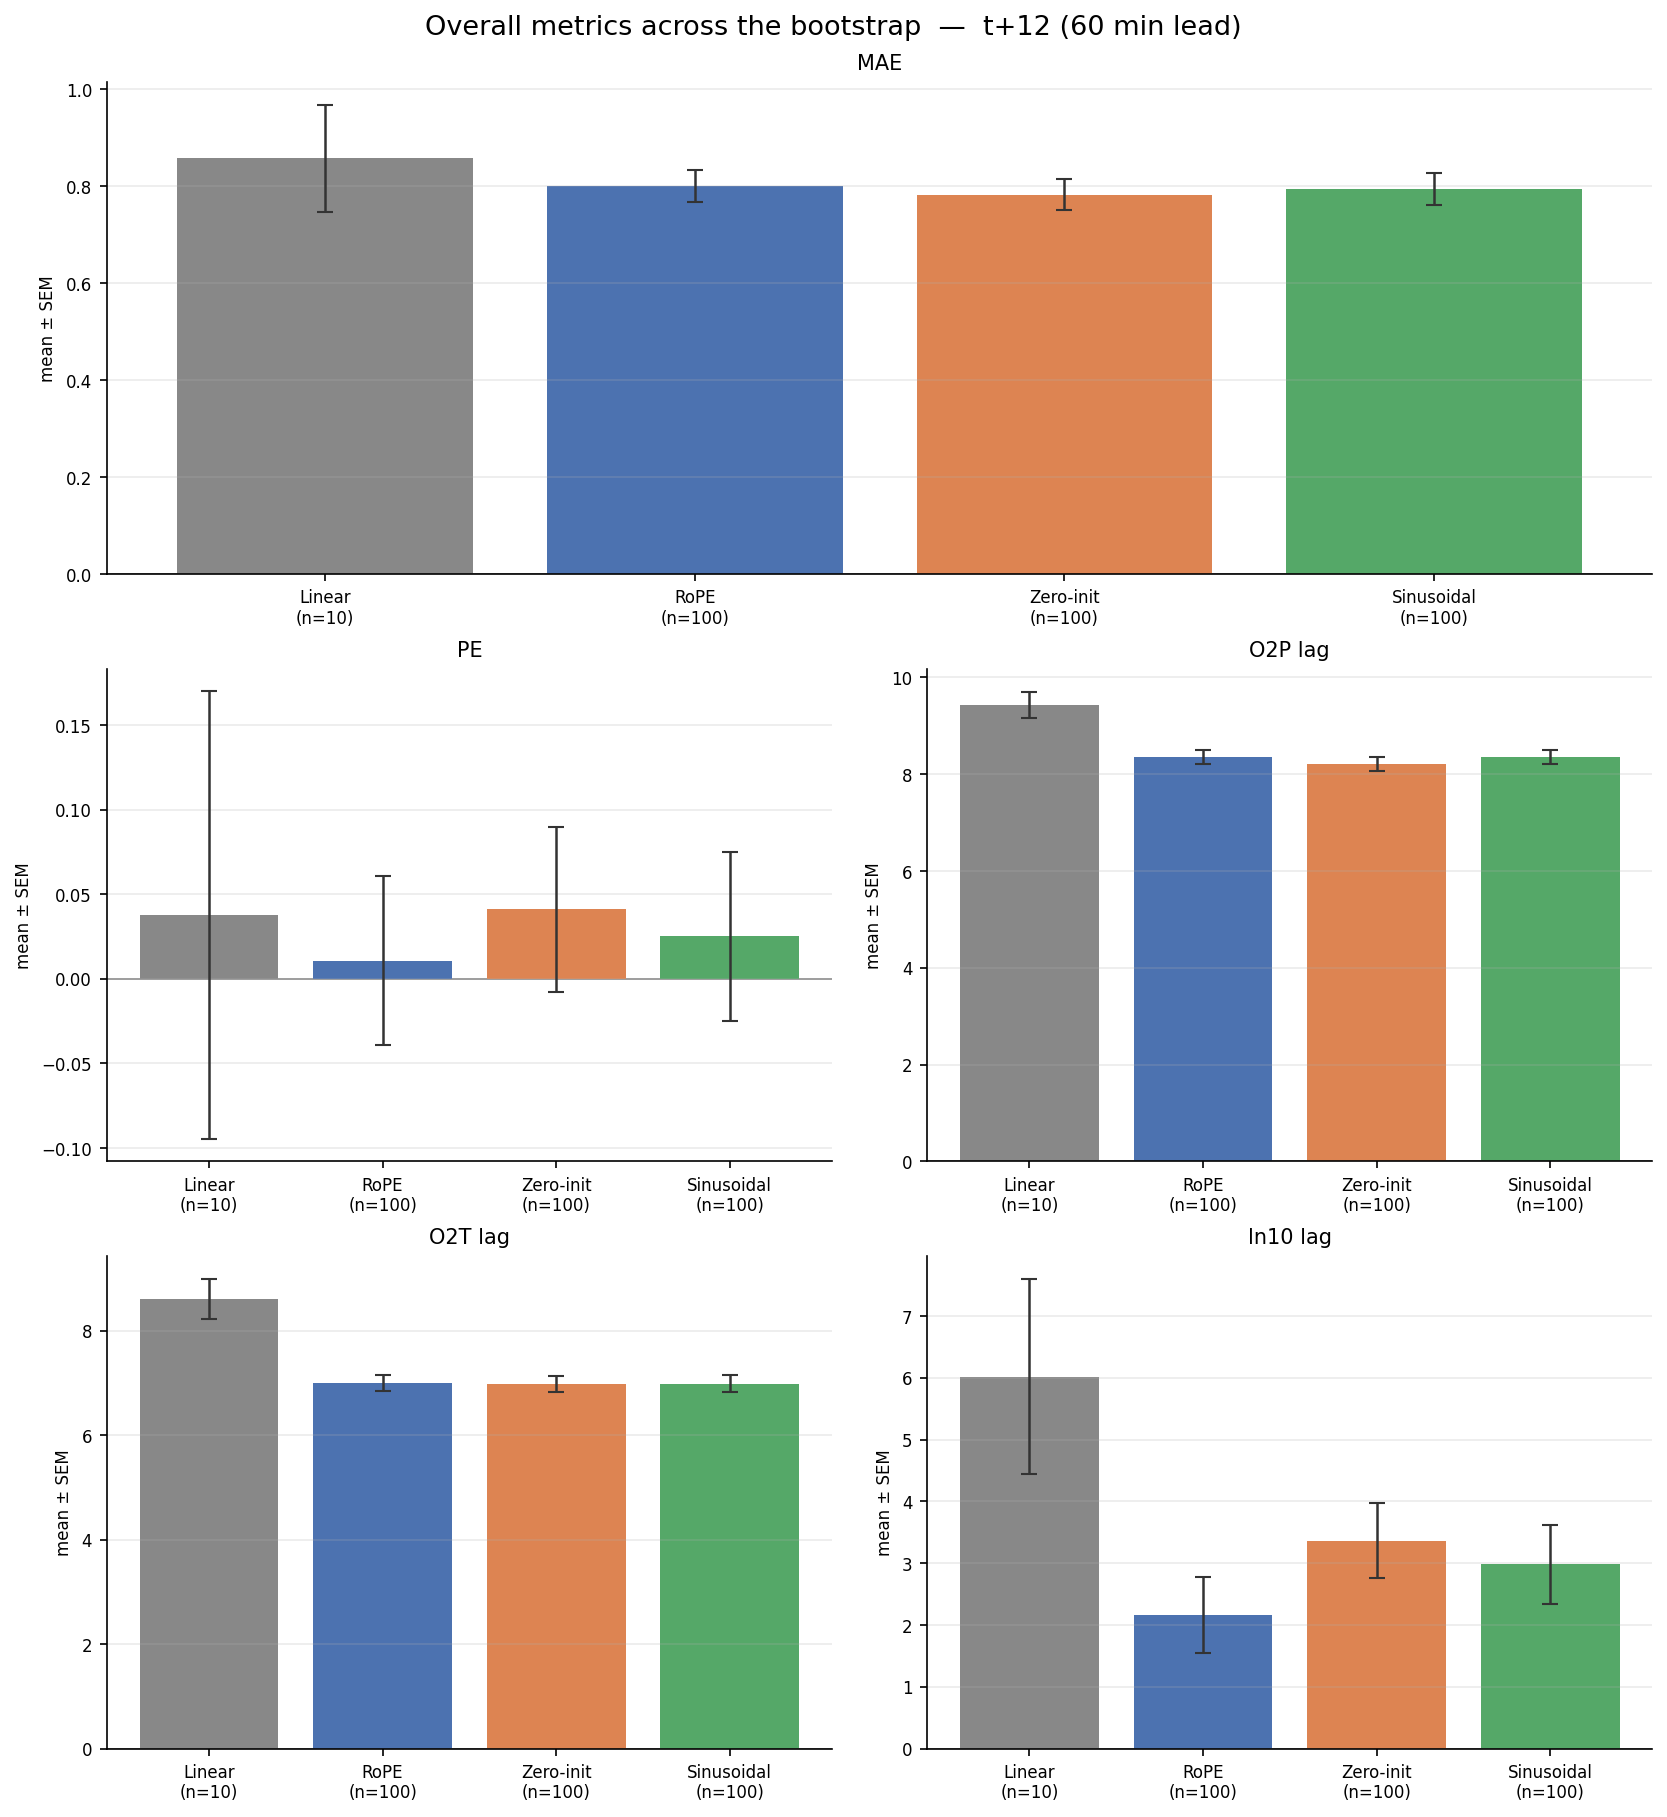
\includegraphics[width=0.7\textwidth]{plots/overall_comparison_t+12.png}
    \caption{Bootstrap of Rope,Sin and Zero init models compared with linear regression  MAE, Lags and Predictive efficiencies with forecasting time of 60 minutes w/ phases TODO add torres nn and rnn}
    \label{fig:sinusoidal_t6_comparison}
\end{figure}
\begin{figure}[H]
    \centering % Centers the image
    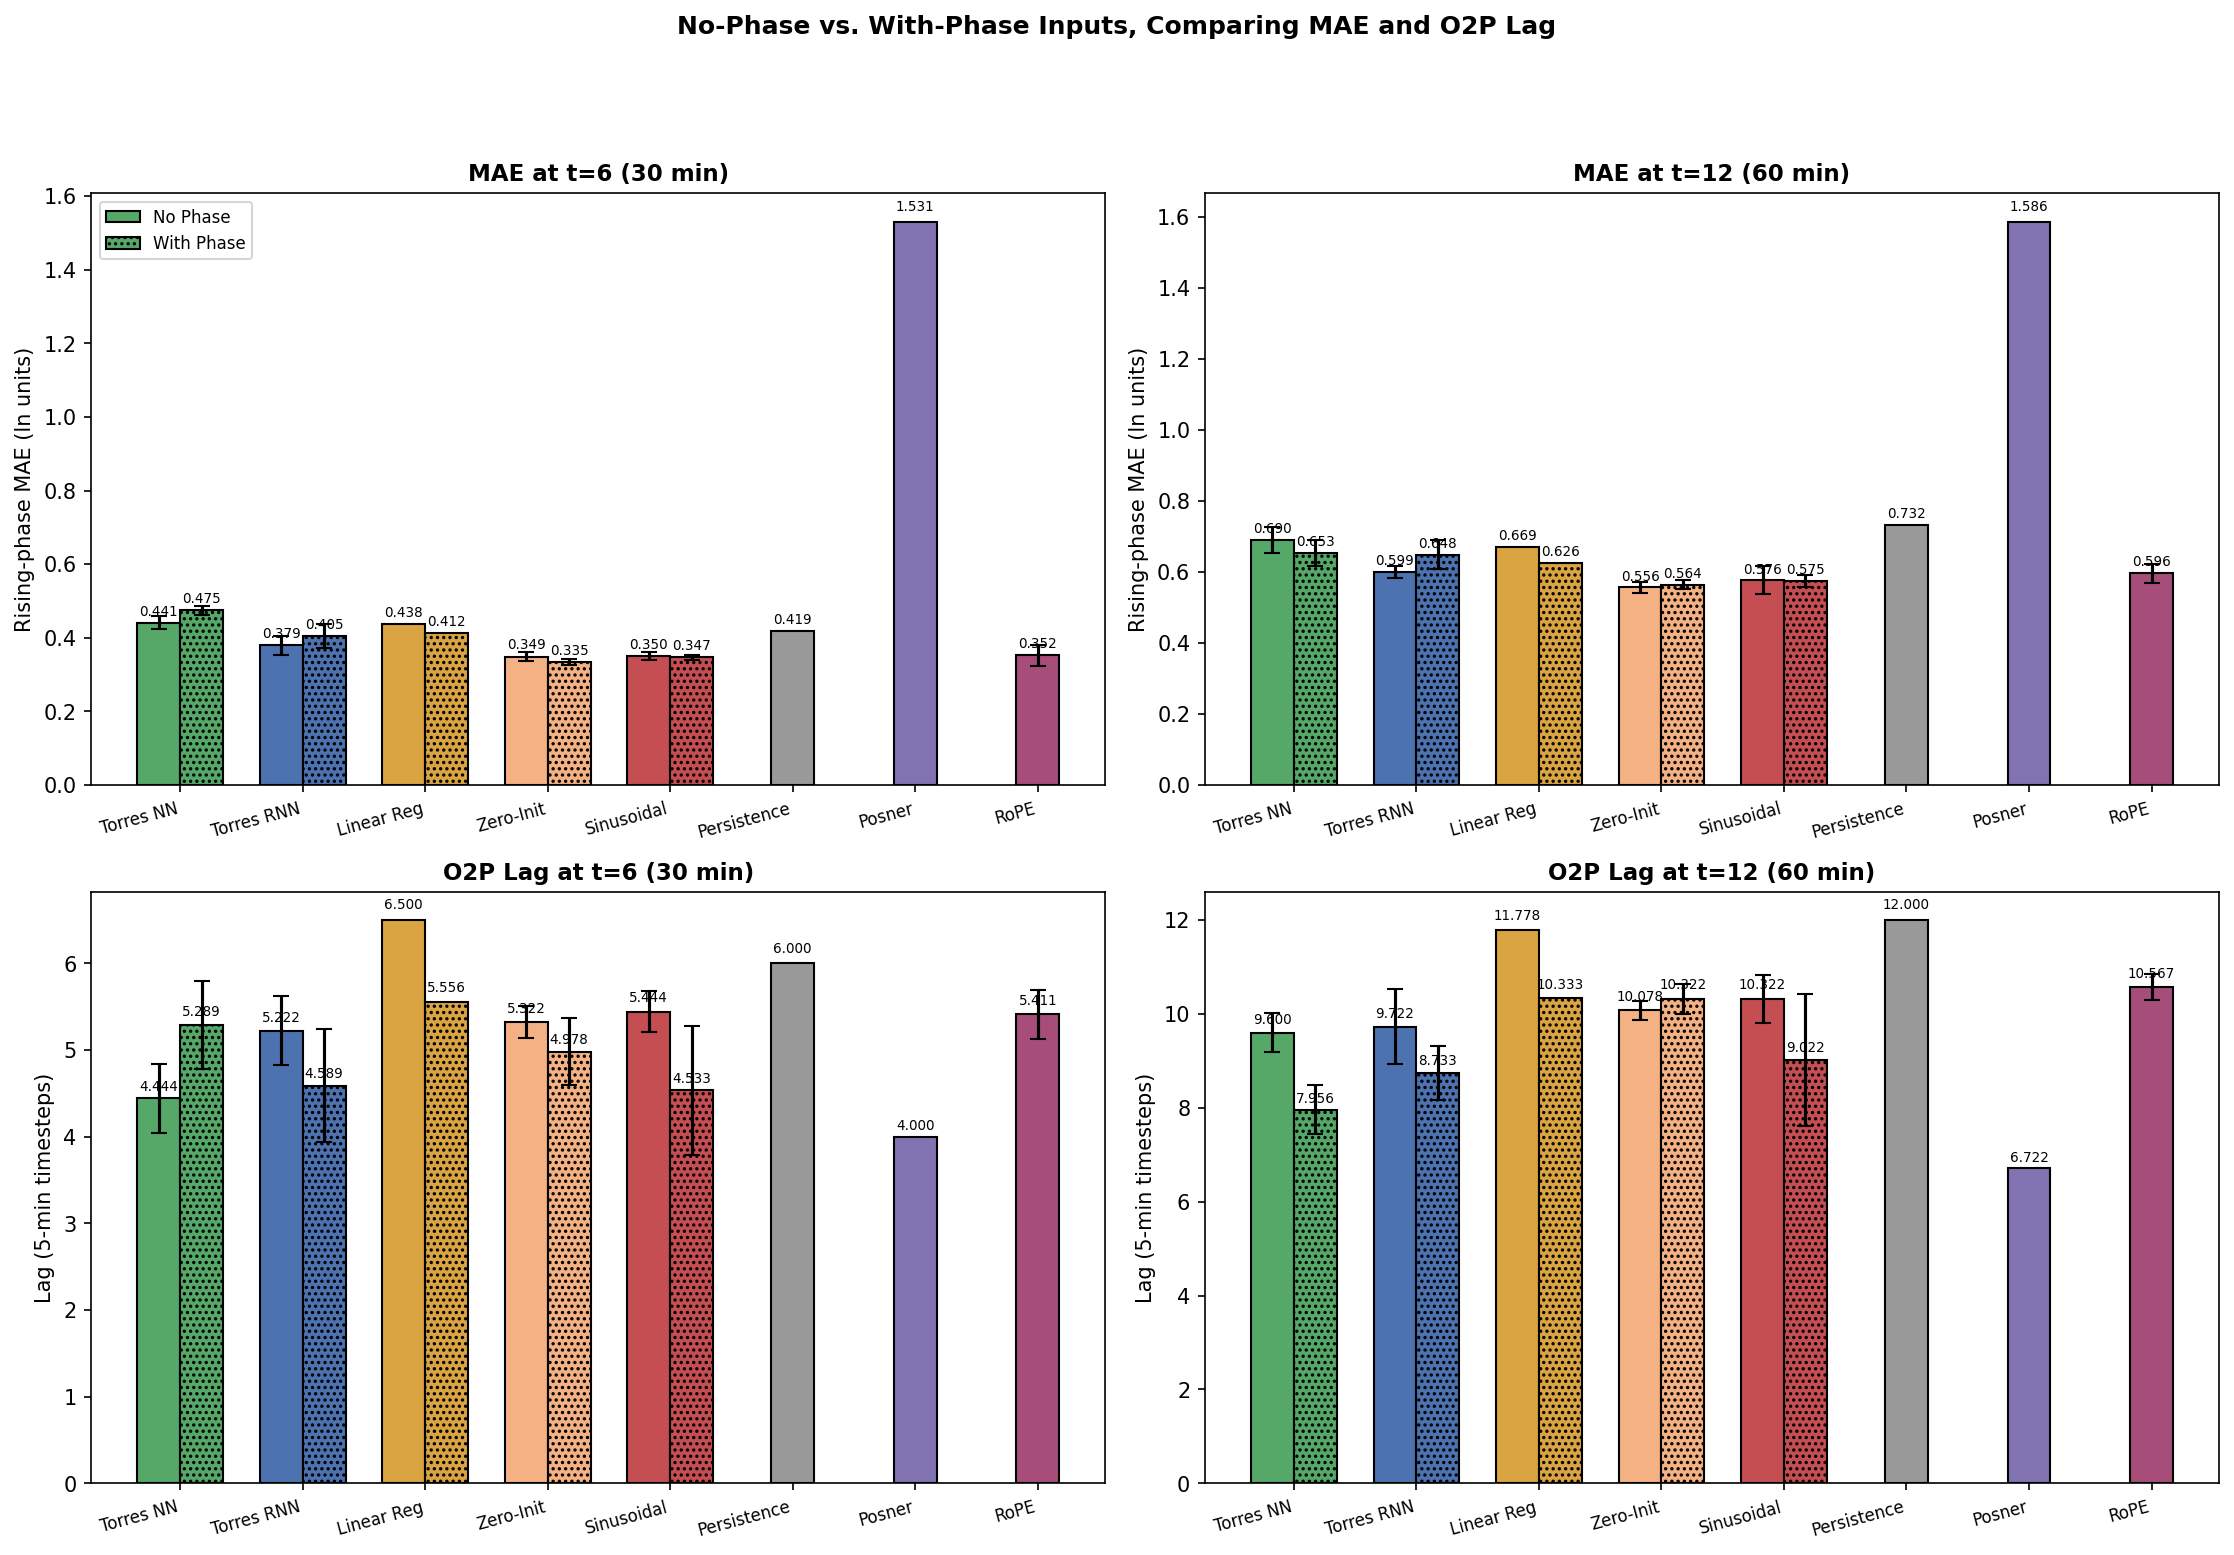
\includegraphics[width=1\textwidth]{plots/mae_lag_phase_comparison.png} % Inserts and resizes image
    \caption{Comparison of MAE and Lag compared to other models} 
    \label{fig: Comparison of lag and MAE between Torres and transformer models} % Label used for referencing
\end{figure}

% \hl{add phases lag and MAE. possibly table. get rid of chart title}


Additional evaluations are needed to score our proton intensity predictions. We evaluate our ability to predict protons $>10 \text{ MeV}$ above $10 \text{ pfu}$ (Threshold to Peak). a warning period is defined  as all consecutive timestamps during which the prediction is above the threshold.

% \begin{table}[H]
\centering

\label{tab:f1_comparison}
\resizebox{\textwidth}{!}{%
\begin{tabular}{l cccc cccc}
\toprule
& \multicolumn{4}{c}{$t+6$} & \multicolumn{4}{c}{$t+12$} \\
\cmidrule(lr){2-5} \cmidrule(lr){6-9}
Method & W & EW & AW & EAW & W & EW & AW & EAW \\
\midrule
Linear Reg   & 0.000 & 0.000 & 0.160 & 0.160 & 0.100 & 0.100 & 0.519 & 0.519 \\
Zero-Init    & \textbf{0.040} (0.055) & \textbf{0.040} (0.055) & 0.613 (0.078) & 0.613 (0.078) & 0.132 (0.079) & \textbf{0.150} (0.120) & 0.732 (0.075) & 0.716 (0.045) \\
Sinusoidal   & 0.038 (0.052) & 0.039 (0.053) & 0.632 (0.068) & 0.632 (0.068) & \textbf{0.137} (0.053) & 0.137 (0.053) & \textbf{0.745} (0.091) & \textbf{0.745} (0.091) \\
RoPE         & 0.036 (0.081) & 0.036 (0.081) & \textbf{0.643} (0.112) & \textbf{0.643} (0.112) & 0.115 (0.079) & 0.115 (0.079) & 0.690 (0.071) & 0.690 (0.071) \\
\bottomrule
\end{tabular}%
}

\caption{Event-detection F1 scores by approach and encoding method, 2-hour alert window (mean $\pm$ std over 5 seeds; Linear Regression is a single deterministic run) No-Phases.}
\end{table}
% \begin{table}[H]
\centering

\label{tab:f1_comparison}
\resizebox{\textwidth}{!}{%
\begin{tabular}{l cccc cccc}
\toprule
& \multicolumn{4}{c}{$t+6$} & \multicolumn{4}{c}{$t+12$} \\
\cmidrule(lr){2-5} \cmidrule(lr){6-9}
Method & W & EW & AW & EAW & W & EW & AW & EAW \\
\midrule
Linear Reg   & 0.348 & 0.364 & 0.562 & 0.581 & 0.250 & 0.261 & 0.706 & 0.788 \\
Torres M1    & 0.30 & 0.48 & 0.62 & 0.76 & 0.16 & \textbf{0.38} & 0.72 & 0.85 \\
Posner       & \textbf{0.56} & \textbf{0.69} & 0.59 & 0.67 & \textbf{0.31} & 0.36 & 0.67 & 0.72 \\
Zero-Init    & 0.309 (0.092) & 0.320 (0.091) & 0.743 (0.055) & 0.761 (0.063) & 0.176 (0.054) & 0.206 (0.040) & 0.782 (0.039) & 0.821 (0.042) \\
Sinusoidal   & 0.350 (0.099) & 0.365 (0.102) & \textbf{0.806} (0.067) & \textbf{0.829} (0.068) & 0.226 (0.043) & 0.238 (0.043) & \textbf{0.824} (0.024) & \textbf{0.852} (0.025) \\
\bottomrule
\end{tabular}%
}

\caption{Event-detection F1 scores by approach and encoding method, 2-hour alert window (mean $\pm$ std over 5 seeds; Linear Regression, Torres M1, and POSNER are single deterministic runs), Phases.}
\end{table}
\begin{figure}[!htbp]
    \centering
    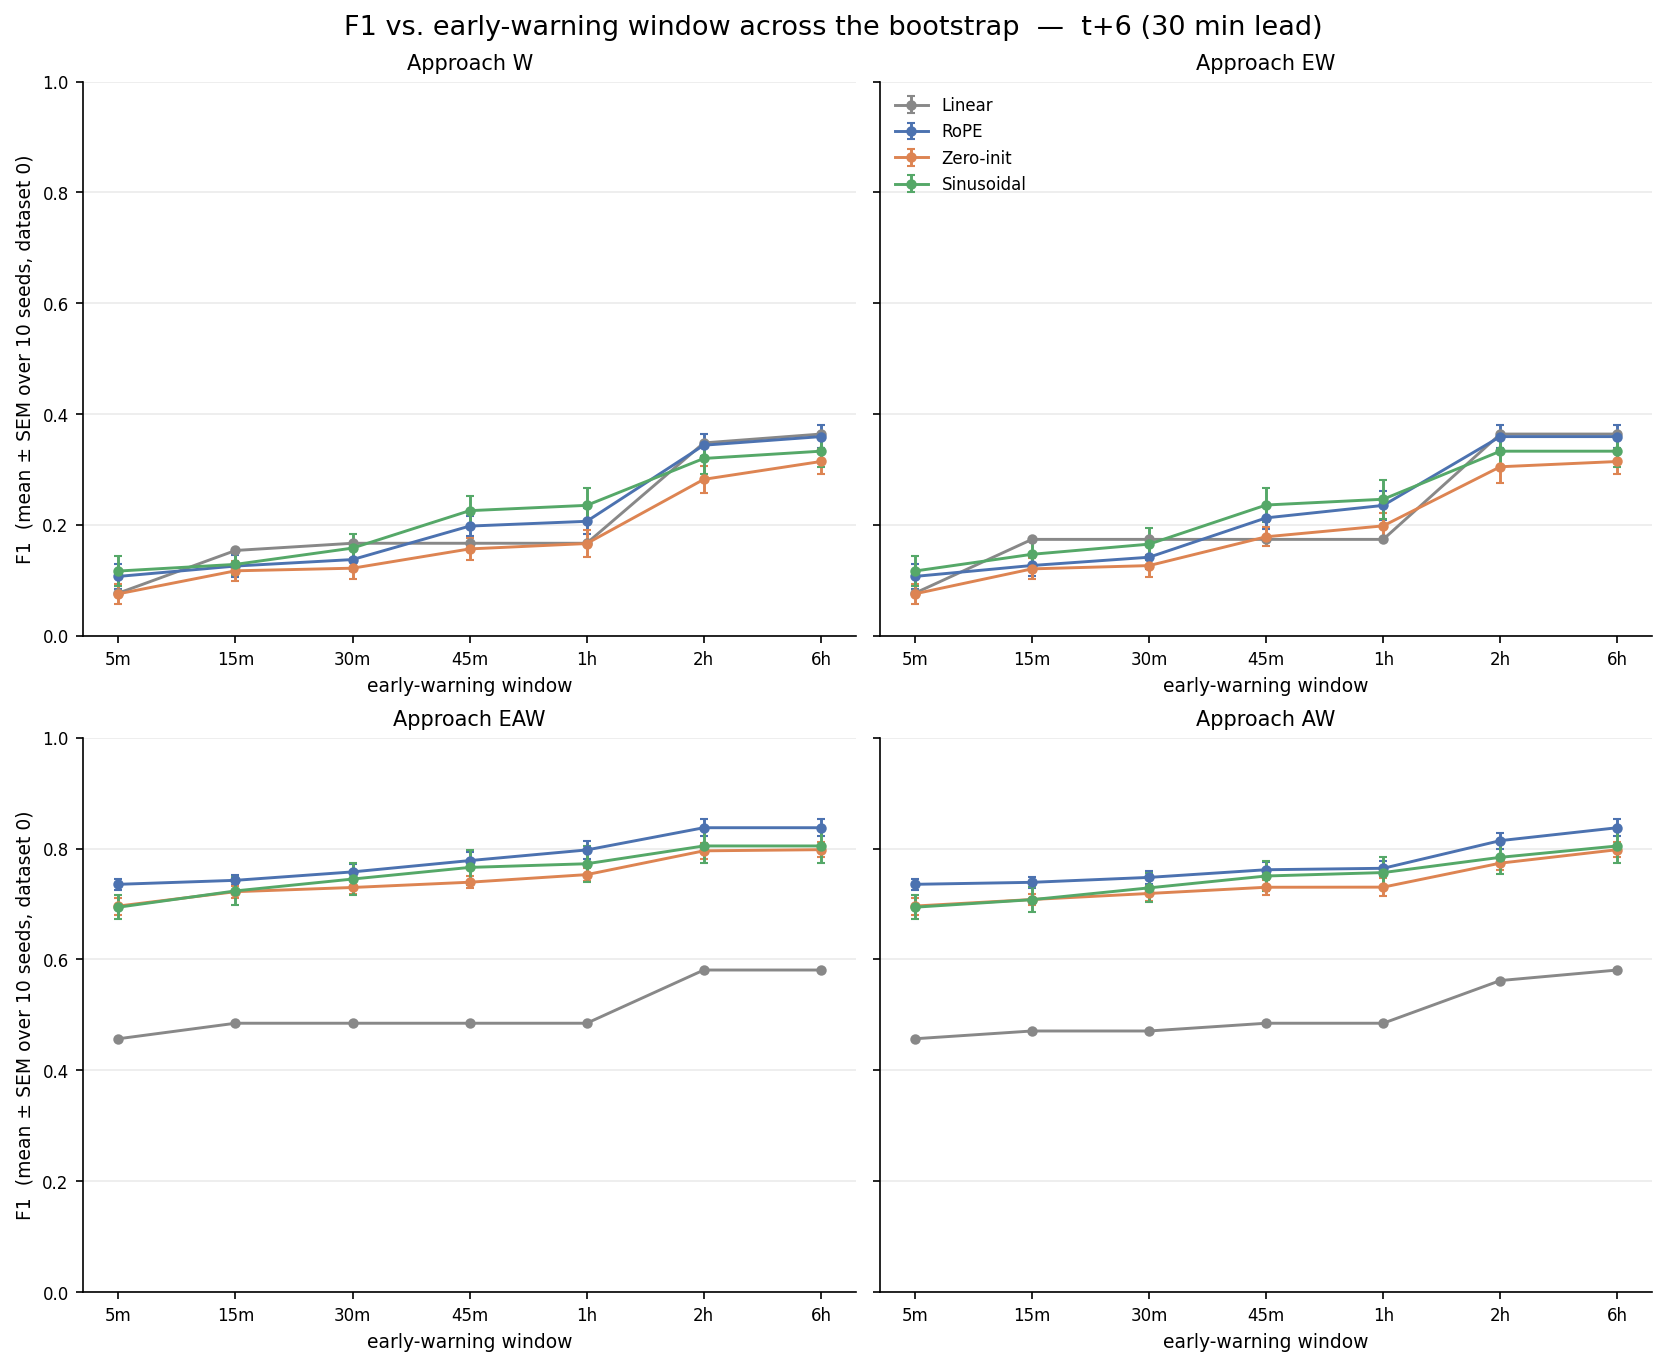
\includegraphics[width=0.7\textwidth]{plots/f1_comparison_t+6.png}
    \caption{Bootstrap of Rope,Sin and Zero init models comparing with linear regression f1 scores 30 minutes w/ phases TODO add torres nn and rnn}
    \label{fig:sinusoidal_t6_comparison}
\end{figure}
\begin{figure}[!htbp]
    \centering
    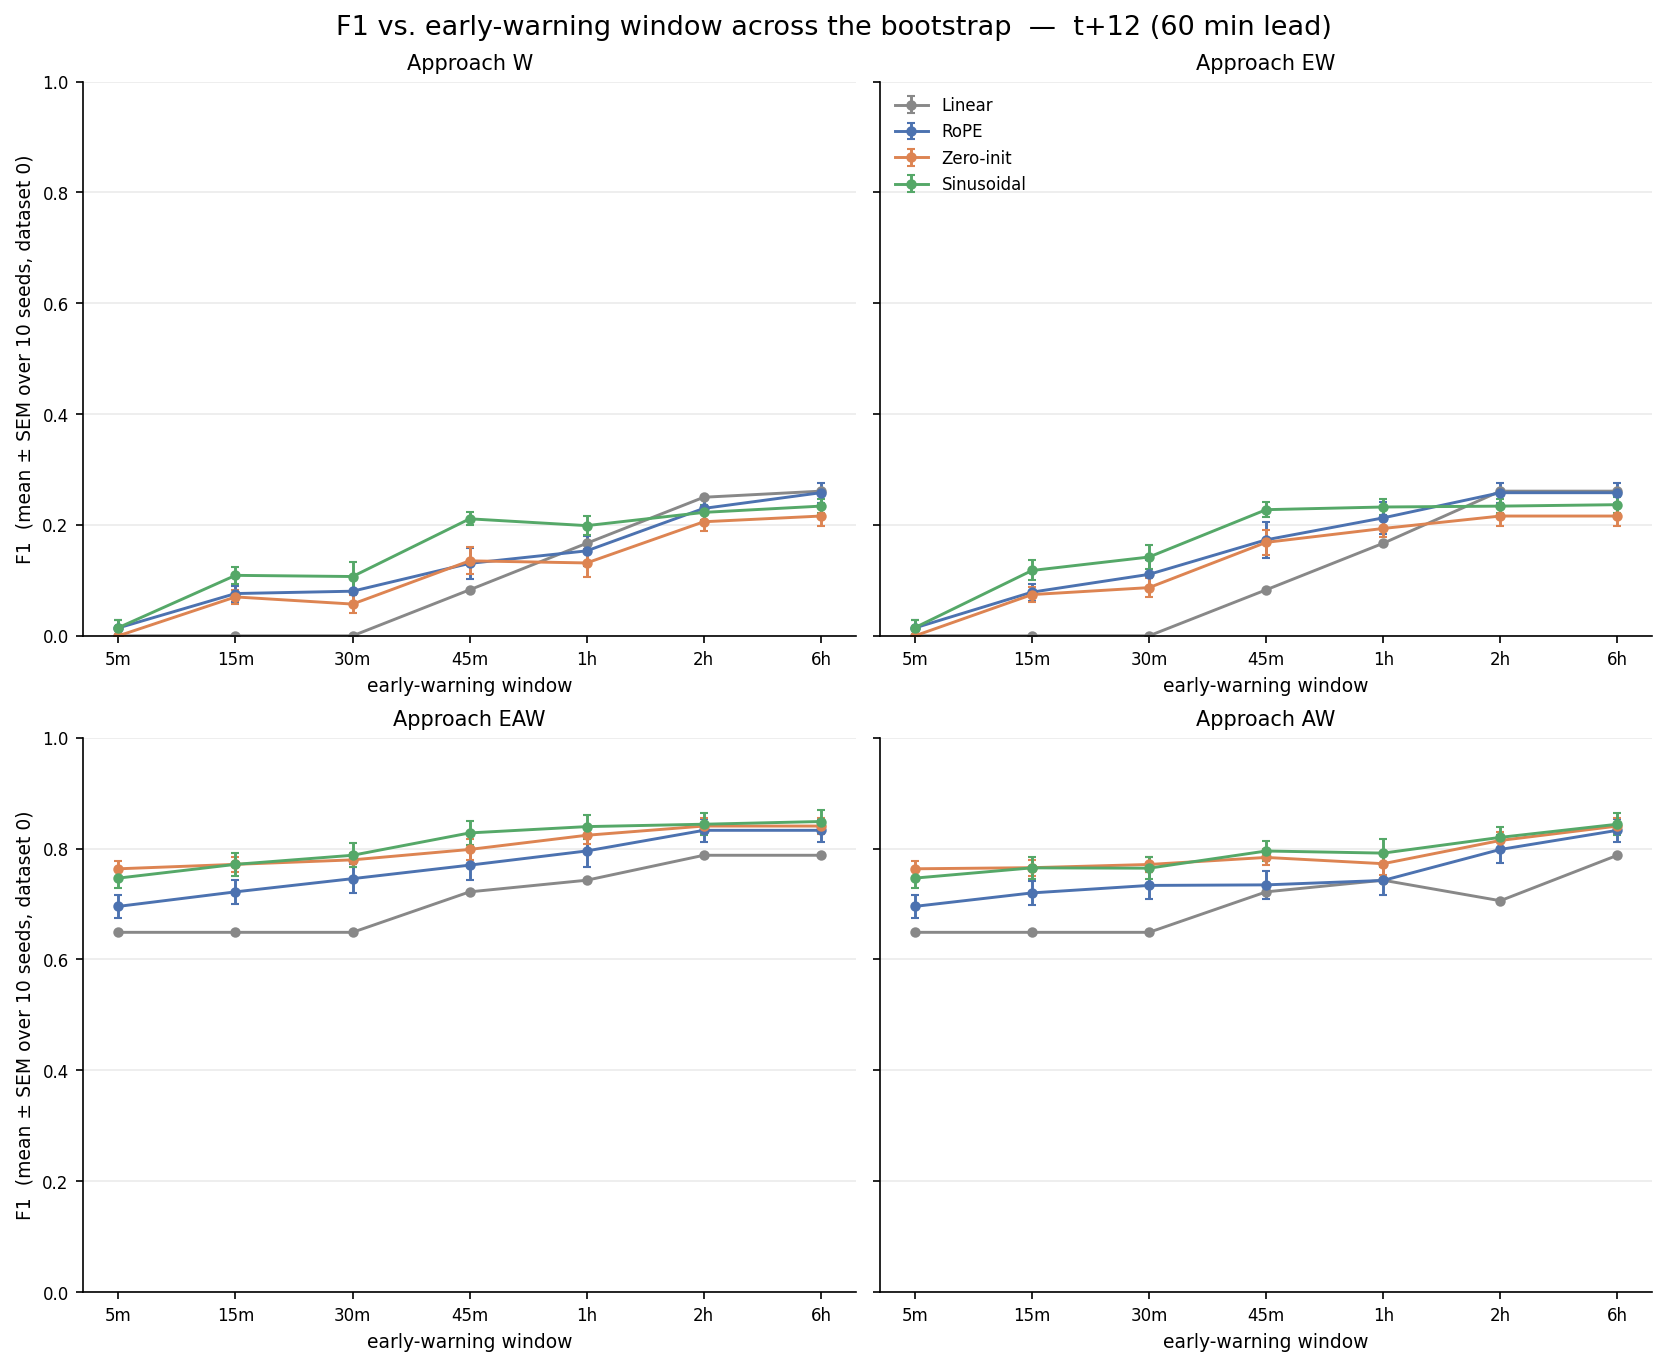
\includegraphics[width=0.7\textwidth]{plots/f1_comparison_t+12.png}
    \caption{Bootstrap of Rope,Sin and Zero init models comparing with linear regression f1 scores 60 minutes w/ phases TODO add torres nn and rnn}
    \label{fig:sinusoidal_t6_comparison}
\end{figure}
\begin{figure}[H]
    \centering % Centers the image
    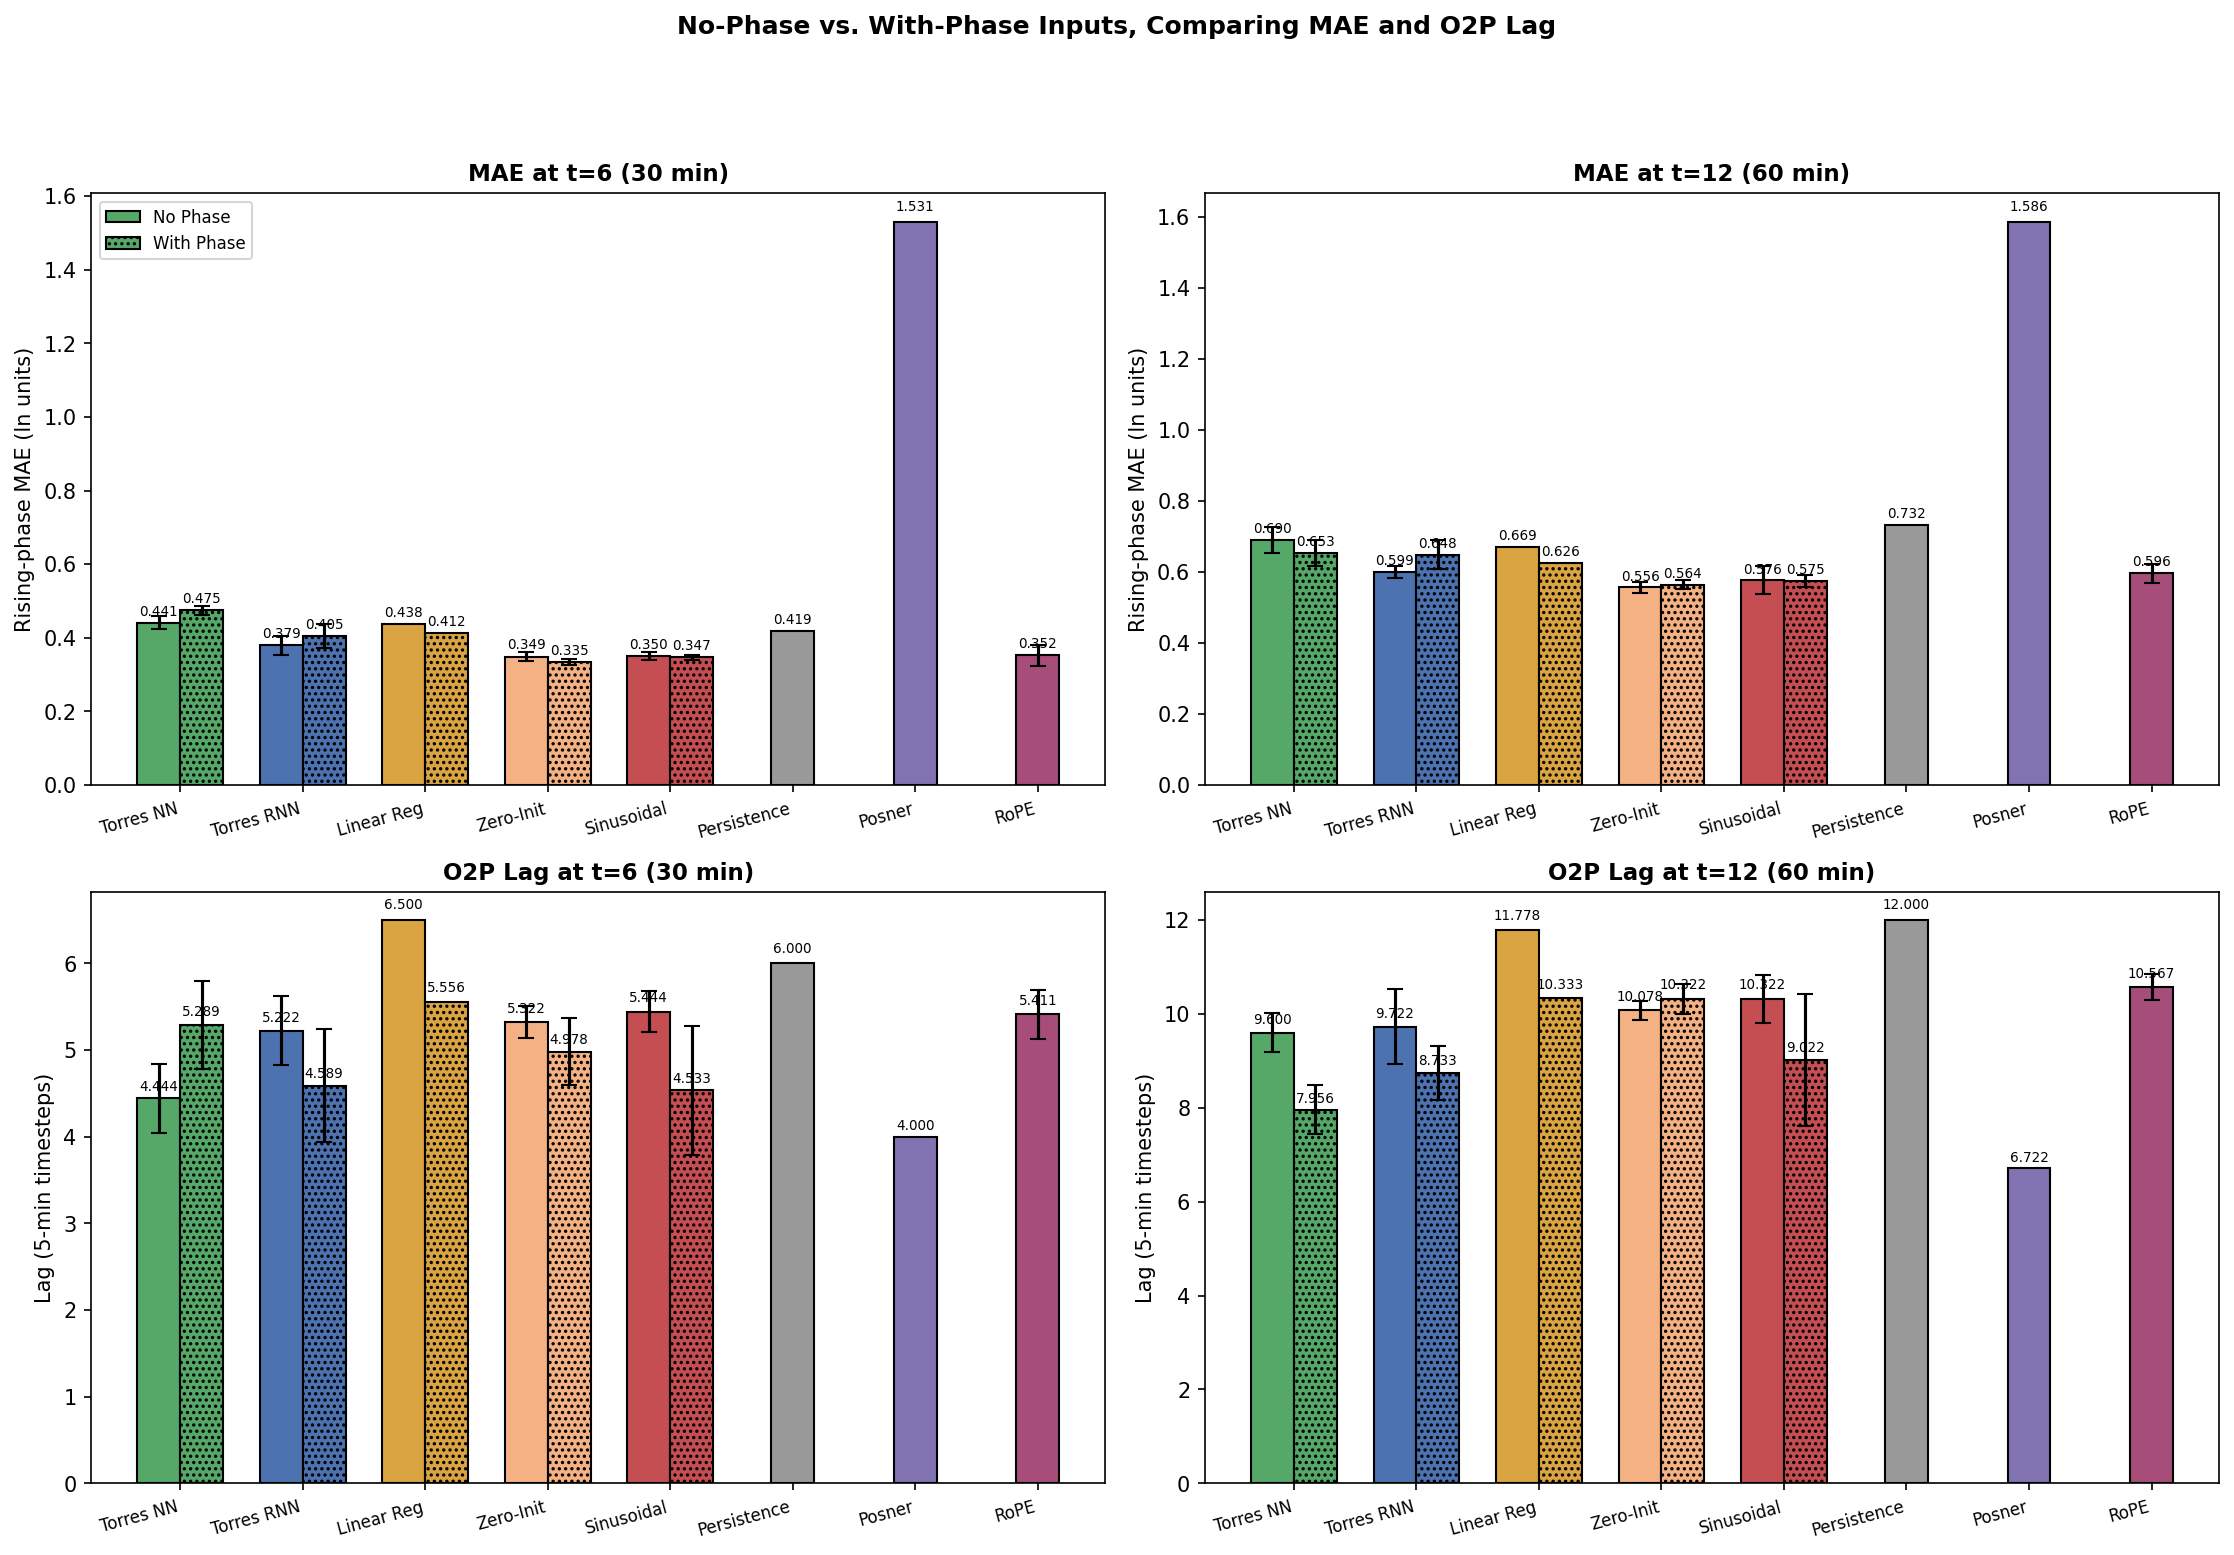
\includegraphics[width=1\textwidth]{plots/mae_lag_phase_comparison.png} % Inserts and resizes image
    \caption{Comparison of MAE and Lag compared to other models} 
    \label{fig: Comparison of lag and MAE between Torres and transformer models} % Label used for referencing
\end{figure}









